%!TEX root = ./hands-on8.tex

\section{About Python}

Python is a programming language invented in the early 1980's by a Dutch programmer named Guido van Rossum who was working at the Dutch National Research Institute for Mathematics and Computer Science.  Python is a high-level programming language with a simple syntax that is easy to learn. The language supports a variety of programming paradigms including procedural programming, object-oriented programming, as well as some functional programming idioms. The name of the language is a whimsical nod toward Monty Python's Flying Circus.

Python has a very active development community. There is a stable core to the language, but new language features are also being developed. Python has an extensive standard library that includes facilities for a wide range of programming tasks. There is a very large user community the provides support and helps to develop an extensive set of third-party libraries. Python is also highly portable -- it is available on pretty much any computing platform you're likely to use. Python is also open-source and free!

\section{Python Resources}

There are many resources available online and in bookstores for learning Python. A few handy resources are listed here:

\begin{itemize}
 \item \href{http://www.python.org/}{Python Website} -- the official website for the programming language.
 \item \href{http://docs.python.org/tutorial/}{The Python Tutorial} -- the `official' Python tutorial.
 \item \href{http://docs.python.org/library/}{Python Library Reference} -- a reference guide to the many modules that come included with Python.
 \item \href{http://greenteapress.com/thinkpython/thinkpython.html}{Think Python: How to Think Like a Computer Scientist} --  a free book that provides an introduction to programming using Python.
\end{itemize}


\section{Starting the Python interpretter}

The Python interpretter can be started in a number of ways. The simplest
way is to open a shell (terminal) and type |python|. You can open a terminal as follows:
%
\begin{itemize}
    \item On a Mac (OS X) run the terminal program available under |Applications > Utilities|
    \item On Windows open up a command prompt, available from |Start Menu > Accessories|. 
\end{itemize}
%

Once you're at the command prompt type the following command:
\begin{bash}
python
\end{bash}
% 
If everything is working correctly you should see something like:
%
\begin{python}
Enthought Python Distribution -- www.enthought.com
Version: 7.2-2 (32-bit)

Python 2.7.2 |EPD 7.2-2 (32-bit)| (default, Sep  7 2011, 09:16:50) 
[GCC 4.0.1 (Apple Inc. build 5493)] on darwin
Type "packages", "demo" or "enthought" for more information.
>>>     
\end{python}
%
If that command didn't work, please see me for further help configuring your Python installation. From within the default
interpretter you can type |Ctrl-d| (Unix, \OSX) , |Ctrl-z| (Windows) or type |quit()| to stop the interpretter and return to the
command line.

For interactive use, the default interpretter isn't very feature rich,
so the Python community has developed a number of GUIs or shell
interfaces that provide more functionality. For this class we will be
using a shell interface called \href{http://ipython.org/}{IPython}. \ipython is one of the tools that was included when you installed the Enthought Python Distribution.

Recent versions of IPython (v0.11) provides both terminal and GUI-based
shells. The EPD installer will place a number of shortcuts on your Start
Menu or in Launchpad on OS X 10.7, including ones that read
|PyLab| and |QtConsole|. These are a terminal based
and GUI based versions of IPython respectively, both of which
automatically load key numerical and plotting libraries. Click on both
of these icons to compare their interfaces.

To get the functionality of |PyLab| from the terminal, run the
following command from your shell:
%
\begin{bash}
ipython --pylab
\end{bash}
%
Again, |Ctrl-d| or |Ctrl-z| will quite t

To get the equivalent of |QtConsole| you can run ipython with
the following arguments:
%
\begin{bash}
ipython qtconsole --pylab
\end{bash}
%
QtConsole is a recent addition to IPython and there may still be bugs to
be sorted out, but it provides some very nice features like `tooltips'
(shows you useful information about functions as you type) and the
ability to embed figures and plots directly into the console, and the
ability to save a console session as a web page (with figures
embedded!).

\subsection{Quick IPython tips}

IPython has a wealth of features, many of which are detailed in its
\href{http://ipython.org/documentation.html}{documentation}. There are
also a number of videos available on the IPython page which demonstrate
some of it's power. Here are a few key features to get you started and
save you time:

\begin{itemize}
\item
  \emph{Don't retype that long command!} --- You can scroll back and
  forth through your previous inputs using the up and down arrow keys
  (or |Ctrl-p| and |Ctrl-n|); once you find what you
  were looking forward you can edit or change it. For even faster
  searching, start to type the beginning of the input and then hit the
  up arrow.
\item
  \emph{Navigate using standard Unix commands} --- IPython lets you use
  standard Unix commands like |ls| and |cd| and
  \lstinline!pwd! to navigate around your file system (even on Windows!)
\item
  \emph{Use \texttt{<Tab>} for command completion} ---
  when your navigating paths or typing function names in you can hit the
  |<Tab>| key and IPython will show you matching functions or
  filenames (depending on context). For example, type
  |cd ./<Tab>| and IPython will show you all the files and
  subdirectories of your current working directory. Type a few of the
  letters of the names of one of the subdirectories and hit
  |<Tab>| again and IPython will complete the name if it finds
  a unique match. Tab completeion allows you to very quickly navigate
  around the file system or enter function names so get the hang of
  using it.
\end{itemize}


\subsection{IP[y] Notebooks}

For most of this class we'll be using a web-browser based `notebook' to interface with Python. This notebook tool, called \ipy, is included with \ipython.   \ipy notebooks are similar to Mathematica notebooks, or Sweave/Knitr documents, in that you can weave together code and text.

To start an \ipy notebook first open up a terminal or command prompt and type the following command:
%
\begin{bash}
ipython notebook --pylab=inline
\end{bash}
%
If \ipython was installed correctly this will open up a new tab or window in your webbrowser, as show in \cref{fig:ipystart}. Click the ``New Notebook" button in the upper right and you'll be presented with an interface like the one show in \cref{fig:ipynotebook}.

\begin{figure}[!ht]
    \centering
    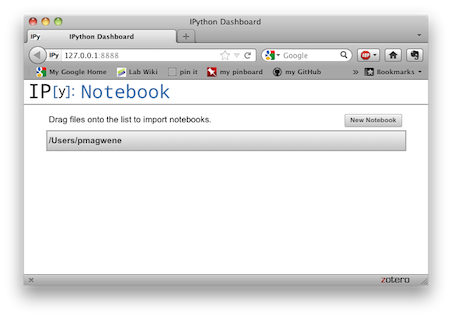
\includegraphics[width=0.5\columnwidth]{./figures/hands-on8/ipy-start.png}
    \caption{The web-browser based \ipy Notebook is a new feature of \ipython, available in version 0.12.}\label{fig:ipystart}
\end{figure}

\begin{figure}[!ht]
    \centering
    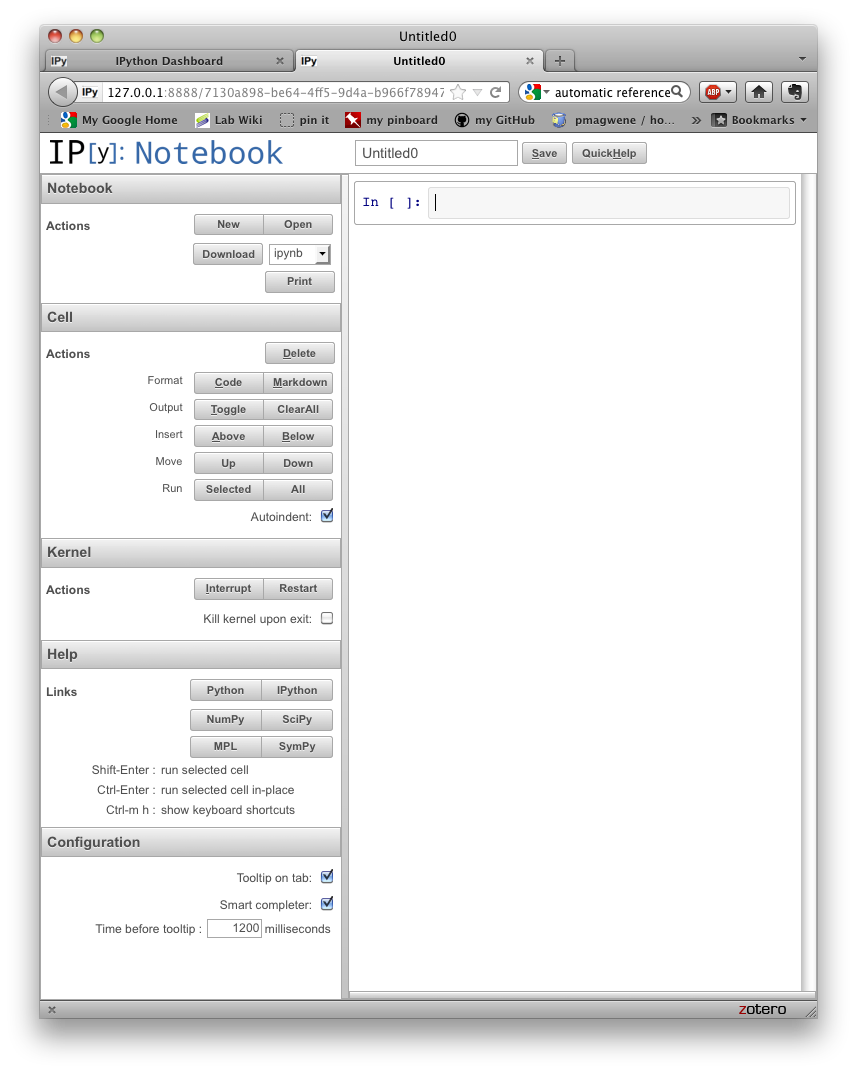
\includegraphics[height=0.5\textheight]{./figures/hands-on8/ipy-interface.png}
    \caption{The \ipy Notebook interface.}\label{fig:ipynotebook}
\end{figure}

\subsection{Entering commands in IP[y] Notebooks}

Unlike the normal Python interpreter, when you hit |Enter| in an \ipy notebook, the commands you enter in a notebook cell are not immediately evaluated. You have to use |Shift-Enter| (hold the |Shift| key while you hit the |Enter| key) when you want a cell to be evaluated.

In the examples that follow, lines that begin with |>>>| indicate lines that you should enter in the \ipy notebook. Lines that follow will indicate the output produced by that command (sometimes the output will be omitted).

\subsection{Exploring some of the power Python}

Let's start off by demonstrating some of the cool things you can do with Python. This will also serve to demonstrate some of the powerful features of the \ipy notebook format. The examples should be fairly self-explanatory; I will defer explanation of specific function calls and the various libraries until later.
%
\begin{python}
>>> x = array([1,2,3,4,5,6,7,8,9,10])
>>> plot(x, x**2)
\end{python}

\begin{alert}
    When entering these lines from inside \ipy, remember to hit |Shift-Enter| to evaluate the commands!
\end{alert}

Now click on the notebook cell with the |plot| command, change it to the following, and hit |Shift-Enter| to re-evaluate the cell.
%
\begin{python}
plot(x, x**2, color='red', marker='o')
xlabel("Length")
ylabel("Area")
title("Length vs. Area for Squares")
\end{python}
%
One of the coolest features of \ipy notebooks is that they allow you to interactively enter some code, evaluate the results, and then go back and fix, edit or change the code and re-evaluate it without having to reload or compile anything. This is particularly useful for interactively creating complex graphics.
%
% \begin{figure}[!ht]
%     \centering
%     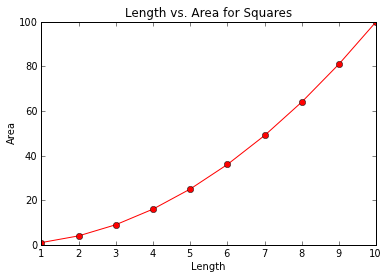
\includegraphics[width=0.75\columnwidth]{fig-simpleplot.png}
%     \caption{A basic plot.}\label{fig:simpleplot}
% \end{figure}

Let's create a more complicated figure, illustrating a histogram of random draws from a normal distribution, compared to the expected probability distribution function (PDF) for a normal distribution with the same parameters:
\begin{python}
mean = 100
sd = 15

# draw 1000 random samples from a normal distn
normaldraw = normal(mean, sd, size=1000)

# draw a histogram
# "normed" means normalize the counts
n, bins, patches = hist(normaldraw, bins=50, normed=True)
xlabel("x")
ylabel("density")

# draw the normal PDF for the same parameters
# evaluated at the bins we used to construct the histogram
y = normpdf(bins, mean, sd)
l = plot(bins, y, "r--", linewidth=2)    
\end{python}
%
This produces the plot shown in \cref{fig:histexample}.
\begin{figure}[!ht]
    \centering
    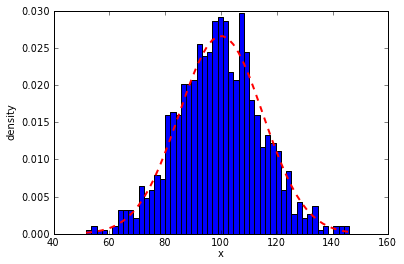
\includegraphics[width=0.5\columnwidth]{./figures/hands-on8/fig-histexample.png}
    \caption{A histrogram created using \ipy and the \matplotlib library.}\label{fig:histexample}
\end{figure}

In this final set of examples we create several representations of the function $z = \cos(x) \sin(y)$.
%
\begin{python}
def f(x,y):
    # multiply by pi/180 to convert degrees to radians
    return cos(x*pi/180) * sin(y*pi/180)

# note we set the upper boundary as 361
# so that 360 get's included
x,y = ogrid[0:361:10, 0:361:10]
z = f(x,y)

# ravel insures the x and y are 1d arrays
# try with 'contour' rather than 'contourf'
p = contourf(ravel(x), ravel(y),z)

lx = xlabel("x (degrees)")
tx = xticks(arange(0,361,45))
ly = ylabel("y (degrees)")
tx = yticks(arange(0,361,45))
\end{python}
%
And the same function represented in 3D, that produces \cref{fig:3dplot}.
%
\begin{python}
from mpl_toolkits.mplot3d import Axes3D
fig = figure()
ax = Axes3D(fig)

# create x,y grid
x,y = meshgrid(arange(0,361,10), arange(0,361,10))
z = f(x,y) # uses fxn f from previous cell
ax.plot_surface(x,y,z,rstride=2,cstride=2,cmap="jet")

# setup axes labels
ax.set_xlabel("x (degrees)")
ax.set_ylabel("y (degrees)")
ax.set_zlabel("z")

# set elevation and azimuth for viewing
ax.view_init(68,-11) 
\end{python}
%
\begin{figure}[!ht]
    \centering
    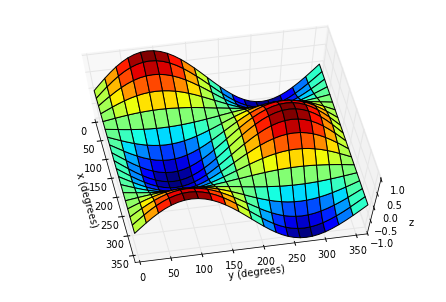
\includegraphics[width=0.5\columnwidth]{./figures/hands-on8/fig-3dplot.png}
    \caption{A 3D representation of $z = \cos(x) \sin(y)$}\label{fig:3dplot}
\end{figure}


% The |plot()| function is not a built-in function in Python, but rather is provided by a plotting library for Python called \href{http://matplotlib.sourceforge.net/}{\matplotlib}. \matplotlib provides powerful 2D and 3D plotting functions that facilitate the production of publication quality figures.

\subsection{Accessing the Documentation}

Python comes with extensive \href{http://docs.python.org/}{HTML documentation}. If you have a network connection, you can access the online documentation for Python (and several other packages) by clicking the appropriate button under ``Help" in the left-hand frame of \ipy. Alternately, you can use the |help()| function (a built-in function in Python), or the |?| command (specific to \ipython):
%
\begin{python}
>>> help(len)
>>> ?len
\end{python}



\section{Using Python as a Calculator}

As with R, the simplest way to use Python is as a fancy calculator.
Let's explore some simple arithmetic operations:
%
\begin{python}
>>> 2 + 10   # this is a comment
12
>>> 2 + 10.3
 12.300000000000001  # 0.3 can't be represented exactly in floating point precision
>>> 2 - 10
-8
>>> 1/2  # integer division
0
>>> 1/2.0  # floating point division
0.5
>>> 2 * 10.0
20.0
>>> 10**2  # raised to the power 2
100
>>> 10**0.5  # raised to a fractional power
3.1622776601683795
>>> (10+2)/(4-5)
-12
>>> (10+2)/4-5  # compare this answer to the one above 
-2
\end{python}
%
In addition to integers and reals (represented as floating points
numbers), Python knows about complex numbers:
%
\begin{python}
>>> 1+2j  # Engineers use 'j' to represent imaginary numbers
(1+2j)
>>> (1 + 2j) + (0 + 3j)
(1+5j)
\end{python}

Some things to remember about mathematical operations in Python:
\begin{itemize}
\item
  Integer and floating point division are not the same in Python.
  Generally you'll want to use floating point numbers.
\item
  The exponentiation operator in Python is |**|
\item
  Be aware that certain operators have precedence over others. For
  example multiplication and division have higher precedence than
  addition and subtraction. Use parentheses to disambiguate potentially
  confusing statements.
\item
  The standard math functions like |cos()| and
  |log()| are not available to the Python interpeter by
  default. To use these functions you'll need to |import| the
  math library as shown below.
\end{itemize}

For example:
%
\begin{python}
>>> 1/2
0
>>> 1/2.0
0.5    
>>> cos(0.5)
Traceback (most recent call last):
  File "<pyshell#2>", line 1, in -toplevel-
    cos(0.5)
NameError: name 'cos' is not defined
>>> import math  # make the math module available
>>> math.cos(0.5) # cos() function in the math module
0.87758256189037276
>>> pi   # pi isn't defined in the default namespace
Traceback (most recent call last):
  File "<pyshell#5>", line 1, in -toplevel-
    pi
NameError: name 'pi' is not defined
>>> math.pi # however pi is defined in math
3.1415926535897931
>>> from math import * # bring everything in the math module into the current namespace
>>> pi
3.1415926535897931
>>> cos(pi)
-1.0
\end{python}

\subsection{Comparison Operators in Python}

The comparison operators in Python work the same was as they do in R
(except they don't work on lists default). Repeat the comparison
excercises given above.

\section{More Data Types in Python}

You've already seen the three basic numeric data types in Python -
integers, floating point numbers, and complex numbers. There are two
other basic data types - Booleans and strings.

Here's some examples of using the Boolean data type:

\begin{python}
>>> x = True
>>> type(x)
<type 'bool'>
>>> y = False
>>> x == y
False
>>> if x is True:
...     print 'Oh yeah!'
... 
Oh yeah!
>>> if y is True:
...     print 'You betcha!'
... else:
...     print 'Sorry, Charlie'
... 
Sorry, Charlie
>>>
\end{python}
%
And some examples of using the string data type:
%
\begin{python}
>>> s1 = 'It was the best of times'
>>> type(s1)
<type 'str'>
>>> s2 = 'it was the worst of times'
>>> s1 + s2
'It was the best of timesit was the worst of times'
>>> s1 + ', ' + s2
'It was the best of times, it was the worst of times'
>>> 'times' in s1
True
>>> s3 = "You can nest 'single quotes' in double quotes"
>>> s4 = 'or "double quotes" in single quotes'
>>> s5 = "but you can't nest "double quotes" in double quotes"
  File "<stdin>", line 1
    s5 = "but you can't nest "double quotes" in double quotes"
                                   ^
SyntaxError: invalid syntax
\end{python}
%
Note that you can use either single or double quotes to specify strings.

\section{Simple data structures in Python: Lists}

Lists are the simplest `built-in' data structure in Python. List
represent ordered collections of arbitrary objects.
%
\begin{python}
>>> l = [2, 4, 6, 8, 'fred']
>>> l
[2, 4, 6, 8, 'fred']
>>> len(l)
5
\end{python}

Python lists are zero-indexed. This means you can access lists elements
|0| to |len(x)-1|.
%
\begin{python}
>>> l[0]
2
>>> l[3]
8
>>> l[5]
Traceback (most recent call last):
  File "<stdin>", line 1, in <module>
IndexError: list index out of range
\end{python}
%
You can use negative indexing to get elements from the end of the list:
\begin{python}
>>> l[-1] # the last element
'fred'
>>> l[-2] # the 2nd to last element
8
>>> l[-3] # ... etc ...
6
\end{python}

Python lists support the notion of `slices' - a continuous sublist of a
larger list. The following code illustrates this concept:
%
\begin{python}
>>> y = range(10)  # our first use of a function!
>>> y
[0, 1, 2, 3, 4, 5, 6, 7, 8, 9]
>>> y[2:8]
[2, 3, 4, 5, 6, 7]
>>> y[2:-1] # the slice
[2, 3, 4, 5, 6, 7, 8]
>>> y[-1:0] # how come this didn't work? 
[]
# slice from last to first, stepping backwards by 2
>>> y[-1:0:-2]  
[9, 7, 5, 3, 1]
\end{python}

\section{Using NumPy arrays}

As mentioned during lecture, Python does not have a built-in data
structure that behaves in quite the same way as do vectors in R.
However, we can get very similar behavior using a library called \numpy.

\numpy does not come with the standard Python distribution, but it does come
as an included package if you use the Enthought Python distribution.
Alternately you can download \numpy from the SciPy project page at:
\url{http://numpy.scipy.org}. The \numpy package comes with documentation and
a tutorial. You can access the documentation at
\url{http://docs.scipy.org/doc/}.

Here's some examples illustrating using of \numpy:
\begin{python}
>>> from numpy import array # a third form of import 
>>> x = array([2,4,6,8,10])
>>> -x
array([ -2,  -4,  -6,  -8, -10])
>>> x ** 2
array([  4,  16,  36,  64, 100])
>>> pi * x # assumes pi is in the current namespace
array([  6.28318531,  12.56637061,  18.84955592,  25.13274123,  31.41592654])
>>> y = array([0, 1, 3, 5, 9])
>>> x + y
array([ 2,  5,  9, 13, 19])
>>> x * y
array([ 0,  4, 18, 40, 90])
>>> z = array([1, 4, 7, 11])
>>> x+z
Traceback (most recent call last):
  File "<stdin>", line 1, in <module>
ValueError: shape mismatch: objects cannot be broadcast to a single shape
\end{python}
%
The last example above shows that, unlike R, \numpy arrays in Python are
not `recycled' if lengths do not match.

Remember that lists and arrays in Python are zero-indexed rather than
one-indexed.
%
\begin{python}
>>> x
array([ 2,  4,  6,  8, 10])
>>> len(x)
5
>>> x[0]
2
>>> x[1]
4
>>> x[4]
10
>>> x[5]

Traceback (most recent call last):
  File "<pyshell#52>", line 1, in -toplevel-
    x[5]
IndexError: index out of bounds
\end{python}

\numpy arrays support the comparison operators and return arrays of
booleans.
\begin{python}
    >>> x < 5 
    array([ True, True, False, False, False], dtype=bool)
    >>> x >= 6 
    array([0, 0, 1, 1, 1])
\end{python}
%
\numpy also supports the combination of comparison and indexing that R vectors
can do. There are also a variety of more complicated indexing functions
available for NumPy; see the
\href{http://docs.scipy.org/doc/numpy/reference/routines.indexing.html}{Indexing Routines} in the Numpy docs.
%
\begin{python}
>>> x[x < 5]
array([2, 4])
>>> x[x >= 6]
array([ 6,  8, 10])
>>> x[(x<4)+(x>6)]  # 'or'
array([ 2,  8, 10])
\end{python}
%
Note that Boolean addition is equivalent to `or' and Boolean
multiplication is equivalent to `and'.

Most of the standard mathematical functions can be applied to NumPy
arrays however you must use the functions defined in the
\numpy module.
%
\begin{python}
>>> x
array([ 2,  4,  6,  8, 10])
>>> import math
>>> math.cos(x)

Traceback (most recent call last):
  File "<pyshell#67>", line 1, in -toplevel-
    math.cos(x)
TypeError: only length-1 arrays can be converted to Python scalars.
>>> import numpy
>>> numpy.cos(x)
array([-0.41614684, -0.65364362,  0.96017029, -0.14550003, -0.83907153])
\end{python}


\section{Writing Functions in Python}

The general form of a Python function is as follows:
%
\begin{python}
def funcname(arg1,arg2):
    # one or more expressions
    return someresult # arbitrary python object (could even be another function)
\end{python}
%
An important thing to remember when writing functions is that Python is
white space sensitive. In Python code indentation indicates scoping
rather than braces. Therefore you need to maintain consistent
indentation. This may surprise those of you who have extensive
programming experience in another language. However, white space
sensitivity contributes significantly to the readability of Python code.
Use a Python aware programmer's editor and it will become second nature
to you after a short while. I recommend you set your editor to
substitute spaces for tabs (4 spaces per tab), as this is the default
convention within the python community.

Here's an example of defining and using a function in the Python
interpreter:
%
\begin{python}
>>> def mypyfunc(x,y):
...     return x**2 + y**2 + 3*x*y
... 
>>> mypyfunc(10,12)
604
>>> a = numpy.arange(1,5,0.5)
>>> b = numpy.arange(2,6,0.5)
>>> mypyfunc(a,b)
array([  11.  ,   19.75,   31.  ,   44.75,   61.  ,   79.75,  101.  ,
        124.75])
>>> a = range(1,5)
>>> b = range(1,5)
>>> mypyfunc(a,b)

Traceback (most recent call last):
  File "<pyshell#52>", line 1, in -toplevel-
    mypyfunc(a,b)
  File "<pyshell#45>", line 2, in mypyfunc
    return x**2 + y**2 + 3*x*y
TypeError: unsupported operand type(s) for ** or pow(): 'list' and 'int'
>>> 
\end{python}
%
Note that this function works for numeric types (\lstinline!ints! and
\lstinline!floats!) as well as \lstinline!numpy.arrays! but not for
simple Python lists. If you wanted to make this function work for lists
as well you could define the function as follows:
%
\begin{python}
>>> def mypyfunc(x,y):
...     x = numpy.array(x)
...     y = numpy.array(y)
...     return x**2 + y**2 + 3*x*y
... 
>>> a
[1, 2, 3, 4]
>>> b
[1, 2, 3, 4]
>>> mypyfunc(a,b)
array([ 5, 20, 45, 80])
\end{python}

\subsection{Putting Python functions in Modules}

As with R, you can define your own Python modules that contain user
defined functions. Using a programmer's text editor, write your
function(s) and save it to a file with a \lstinline!.py! extension in a
directory in your PYTHONPATH (see below).

\begin{python}
# functions defined in vecgeom.py
import numpy

def veclength(x):
    """Calculate length of a vector x.""" 
    x = numpy.array(x)
    return numpy.sqrt(numpy.dot(x,x))


def unitvector(x):
    """Return a unit vector in the same direction as x."""
    x = numpy.array(x)
    return x/veclength(x)
\end{python}
%
To access your function use an \lstinline!import! statement:
%
\begin{python}
>>> import vecgeom
>>> x = [-3,-3,-1,-1,0,0,1,2,2,3]
>>> help(vecgeom.veclength)
Help on function veclength in module vecgeom:

veclength(x)
    Calculate length of a vector x.

>>> vecgeom.veclength(x)
6.164414002968976
# import all fxns from the vecgeom module
>>> from vecgeom import * 
>>> print vecgeom.unitvector(x)
[-0.48666426 -0.48666426 -0.16222142 -0.16222142  0.          0.   
     0.16222142  0.32444284  0.32444284  0.48666426]
\end{python}

\section{Setting the PYTHONPATH}

Like the operating system, Python searches a set of default directories whenever you ask it to load a specific module.  Python knows where to find all of it's base modules, and a well written package will install it's files into one of the standard locations.

To see the directories that your Python installation searches by default try the following commands in the Python interpreter (your output will be different):
%
\begin{python}
>>> import sys
>>> import sys
>>> sys.path
['', '/Library/Frameworks/Python.framework/Versions/7.1/bin', '/Users/pmagwene', 
'/Users/pmagwene/synchronized/pyth', '/Users/pmagwene/pytest', 
... output truncated ...
\end{python}

For your own code it's useful to setup a separate directory. Create a directory called |pycode| in your home directory. In order for Python to "see" the code in this directory you must add it to your |PYTHONPATH|.

To temporarily add a new directory to |sys.path|:
\begin{python}
>>> sys.path.append('/Users/pmagwene/pycode') # substitute the path to the directory you used
>>> print sys.path
['', '/Library/Frameworks/Python.framework/Versions/7.1/bin', '/Users/pmagwene', 
'/Users/pmagwene/synchronized/pyth', '/Users/pmagwene/pytest', 
... output truncated...
'/Users/pmagwene/pycode']
\end{python}

This change applies only to your current interpreter and lasts until you close the interactive prompt. To make persistent changes to the Python seach path you need to create an environment variable called |PYTHONPATH| and add the desired directories.  You do this the same way you set your system |PATH|, but modify your shell initialization file (Unix or OS X) or using the System Properties tool in the control panel to create a new environment variable (Windows). For example, on OS X add the following line to your |.bash_profile| (found in your home directory, create it if doesn't already exist):
%
\begin{bash}
export PYTHONPATH=$PYTHONPATH:$HOME/pycode   
\end{bash}
%
If you are keeping your Bio723 code somewhere other than |~/pycode| than change the location as needed. To have this change take effect, start a new Terminal window or re-start \ipy.

For more info on setting PATH variables see: \url{https://github.com/pmagwene/Bio313/wiki/setting-paths}.

\section{Vector Operations in Python}

The Python equivalent of the R code above is:
%
\begin{python}
>>> import numpy
>>> x = numpy.arange(start=1, stop=16, step=1)
>>> y = numpy.arange(10,25) # default step = 1
>>> x
array([ 1,  2,  3,  4,  5,  6,  7,  8,  9, 10, 11, 12, 13, 14, 15])
>>> y
array([10, 11, 12, 13, 14, 15, 16, 17, 18, 19, 20, 21, 22, 23, 24])
>>> x+y
array([11, 13, 15, 17, 19, 21, 23, 25, 27, 29, 31, 33, 35, 37, 39])
>>> x-y
array([-9, -9, -9, -9, -9, -9, -9, -9, -9, -9, -9, -9, -9, -9, -9])
>>> 3*x
array([ 3,  6,  9, 12, 15, 18, 21, 24, 27, 30, 33, 36, 39, 42, 45])
>>> z = numpy.dot(x,x) # no built-in dot operator, but a dot fxn in numpy
>>> z
1240
\end{python}
%
Note the use of the \lstinline!numpy.arange()! function.
\lstinline!numpy.arange()! works like R's \lstinline!sequence()!
function and it returns a Numpy array. However, notice that the values
go up to but don't include the specified \lstinline!stop! value. Use
\lstinline!help()! to lookup the documentation for
\lstinline!numpy.arange()!. Python also includes a \lstinline!range()!
function that generates a regular sequence as a Python list object. The
\lstinline!range()! function has \lstinline!start!, \lstinline!stop!,
and \lstinline!step! arguments but these can only be integers. Here are
some additional examples of the use of \lstinline!arange()! and
\lstinline!range()!:

\begin{python}
>>> z = numpy.arange(1,5,0.5) 
>>> z
array([ 1. ,  1.5,  2. ,  2.5,  3. ,  3.5,  4. ,  4.5])
>>> range(1,20,2)
[1, 3, 5, 7, 9, 11, 13, 15, 17, 19]
>>> range(1,5,0.5)
Traceback (most recent call last):
  File "<stdin>", line 1, in <module>
TypeError: range() integer step argument expected, got float.
\end{python}



\section{Matrices in Python}

Matrices in Python are created are created using the
\lstinline!Numeric.array()! function. In Python you need to be a little
more aware of the type of the arrays that you create. If the argument
you pass to the \lstinline!array()! function is composed only of
integers than Numeric will assume you want an integer matrix which has
consequences in terms of operations like those illustrated below. To
make sure you're matrix has floating type values you can use the
argument \lstinline!typecode=Numeric.Float!.

\begin{python}
>>> import numpy as np # I'm 'aliasing' the name so I can type 'np' instead of 'numpy'
>>> array = np.array # setup another alias
>>> X = array(range(1,13))
>>> X
array([ 1,  2,  3,  4,  5,  6,  7,  8,  9, 10, 11, 12])
>>> X.shape = (4,3) # rows, columns
>>> X
array([[ 1,  2,  3],
       [ 4,  5,  6],
       [ 7,  8,  9],
       [10, 11, 12]])
>>> 1/X # probably not what you expected
array([[1, 0, 0],
       [0, 0, 0],
       [0, 0, 0],
       [0, 0, 0]])
>>> X = array(range(1,13), dtype=np.float)
>>> X.shape = 4,3
>>> X
array([[  1.,   2.,   3.],
       [  4.,   5.,   6.],
       [  7.,   8.,   9.],
       [ 10.,  11.,  12.]])
>>> 1/X # that's more like it
array([[ 1.        ,  0.5       ,  0.33333333],
       [ 0.25      ,  0.2       ,  0.16666667],
       [ 0.14285714,  0.125     ,  0.11111111],
       [ 0.1       ,  0.09090909,  0.08333333]])
>>> X
array([[  1.,   2.,   3.],
       [  4.,   5.,   6.],
       [  7.,   8.,   9.],
       [ 10.,  11.,  12.]])
>>> X + X
array([[  2.,   4.,   6.],
       [  8.,  10.,  12.],
       [ 14.,  16.,  18.],
       [ 20.,  22.,  24.]])
>>> X - X
array([[ 0.,  0.,  0.],
       [ 0.,  0.,  0.],
       [ 0.,  0.,  0.],
       [ 0.,  0.,  0.]])
>>> np.dot(X,np.transpose(X)) # dot fxn in numpy gives matrix multiplication for arrays
array([[  14.,   32.,   50.,   68.],
       [  32.,   77.,  122.,  167.],
       [  50.,  122.,  194.,  266.],
       [  68.,  167.,  266.,  365.]])
>>> np.identity(4)
array([[1, 0, 0, 0],
       [0, 1, 0, 0],
       [0, 0, 1, 0],
       [0, 0, 0, 1]])
>>> np.sqrt(X)
array([[ 1.        ,  1.41421356,  1.73205081],
       [ 2.        ,  2.23606798,  2.44948974],
       [ 2.64575131,  2.82842712,  3.        ],
       [ 3.16227766,  3.31662479,  3.46410162]])
>>> np.cos(X)
array([[ 0.54030231, -0.41614684, -0.9899925 ],
       [-0.65364362,  0.28366219,  0.96017029],
       [ 0.75390225, -0.14550003, -0.91113026],
       [-0.83907153,  0.0044257 ,  0.84385396]])
\end{python}

The code above also demonstrated the Numpy functions \lstinline!dot()!,
\lstinline!transpose()! and \lstinline!identity()!. Note too that Numpy
has a variety of functions such as \lstinline!sqrt()!and
\lstinline!cos()! that work on an element-wise basis.

Indexing of arrays in Numpy is demonstrated below. You'll see that
Python arrays support `slicing' operations. For more on slicing and
other array basics see the Numpy documentation at
\href{http://docs.scipy.org/doc/}{http://docs.scipy.org/doc/}.

\begin{python}
>>> X
array([[  1.,   2.,   3.],
       [  4.,   5.,   6.],
       [  7.,   8.,   9.],
       [ 10.,  11.,  12.]])
>>> X[0,0] # get the 0th row, 0th column (remember that Python sequences are zero-indexed!)
1.0
>>> X[3,0] # get the fourth row, 1st column
10.0
>>> X[:2,:2]  # an example of slicing, get the first two columns and rows (i.e. indices 0 and 1)
array([[ 1.,  2.],
       [ 4.,  5.]])
>>> X[1:,:2] # get everything after the 0th row and  the first two columns
array([[  4.,   5.],
       [  7.,   8.],
       [ 10.,  11.]])
\end{python}
To calculate matrix inverses in Python you need to import the
\lstinline!numpy.linalg! package.

\begin{python}
>>> import numpy.linalg as la
>>> import numpy.random as ra  # for matrices with elements from random distributions
>>> C = ra.normal(loc=0,scale=1,size=(4,4)) # do help(ra.normal) for explanation of argumnets
>>> C
array([[ 0.79525679,  1.11730719, -2.19257712, -0.06289276],
       [ 0.7087366 ,  0.70574975, -1.51599336, -0.90360945],
       [-0.33845153, -0.20109722, -0.75245988, -0.56027025],
       [-0.51692665,  0.59972543,  1.55562234,  1.88639367]])
>>> Cinv = la.inv(C)
>>> np.dot(C, Cinv) # again result is approx the identity matrix due to floating point precision
array([[ 1.00000000e+000, -5.55111512e-017, -6.93889390e-017,  2.94902991e-017],
       [ 1.11022302e-016,  1.00000000e+000, -1.11022302e-016, -5.55111512e-017],
       [ 1.11022302e-016, -2.22044605e-016,  1.00000000e+000,  2.77555756e-017],
       [ 0.00000000e+000, -4.44089210e-016,  0.00000000e+000,  1.00000000e+000]])
>>> print np.array2string(np.dot(C,Cinv),precision=2, suppress_small=True)
[[ 1. -0.  0.  0.]
 [-0.  1.  0.  0.]
 [ 0.  0.  1.  0.]
 [-0. -0. -0.  1.]]
\end{python}




\section{Plotting in Python}

Python doesn't have any `native' data plotting tools but there are a
variety of packages that provide tools for visualizing data. The Matplotlib package is the de facto standard for producing
publication quality scientific graphics in Python. Matplotlib is
included with the EPD and was automatically pulled into the interpretter
namespace if you're using the \ipython |--pylab| option. If you want to explore the full power of Matplotlib check out the example
gallery and the documentation at
\url{http://matplotlib.sourceforge.net/}.

\subsection{Basic plots using matplotib}

If you invoked the Ipython shell using the pylab option than most of the
basic matplotlib functions are already available to you. If not, import
them as so:

\begin{python}
>>> from pylab import * # only necessary if not using pylab
>>> import numpy as np # go ahead and import numpy as well, using an alias

# load the turtle data using the numpy.loadtxt function 
# skipping the first row (header) and the first column 
>>> turt = np.loadtxt('turtles.txt', skiprows=1, 
                      usecols=(1,2,3))
>>> turt.shape
(48, 3)
# draw bivariate scatter plot
>>> scatter(turt[:,0], turt[:,1])
# give the axes some labels and a title for the plot
>>> xlabel('Length')
>>> ylabel('Width')
>>> title('Turtle morphometry')
\end{python}

Here's another example using the yeast expression data set:
%
\begin{python}
>>> data = np.loadtxt('yeast-subnetwork-clean.txt',skiprows=1,usecols=range(1,16))
>>> data.shape   # check the dimensions of the resulting matrix
(173, 15)
\end{python}
The \lstinline!skiprows! argument tells the function how many rows in
the data file you want to skip. In this case we skipped only the first
row which gives the variable names. The \lstinline!usecols! arguments
specificies which columns from the data file to use. Here we skipped the
first (zeroth) column which had the names of the conditions. The usecols
\lstinline!loadtxt! works when there is no missing data. Use
\lstinline!numpy.genfromtxt! instead when there are missing values. For
a full tutorial on how to use the \lstinline!numpy.genfromtxt! function
see
\url{http://docs.scipy.org/doc/numpy/user/basics.io.genfromtxt.html}.

\subsubsection{Histograms in Matplotlib}

Matplotlib has a histogram drawing function. Here's how to use it:
%
\begin{python}
>>> hist? # in Ipython calls the help function
>>> h = hist(data[:,0]) # plot a histogram of the first variable (column) in our data set
>>> clf() # clear the plot window, don't need this if you closed the plot window
>>> h = hist(data[:,0], bins=20) # plot histogram w/20 bins
>>> h = hist(data[:,:2])  # histograms of the first two variables    
\end{python}

There's no built in density plot function, but we can create a function
that will do the necessary calculations for us to create our own density
plot. This uses a kernel density estimator function in the scipy library
(included with EPD). Put the following code in a file called
\lstinline!myplots.py! somewhere on your \lstinline!PYTHONPATH!:
%
\begin{python}
# myplots.py

import numpy as np
from scipy import stats

def density_trace(x):
    kde = stats.gaussian_kde(x)
    xmin,xmax = min(x), max(x)
    xspan = xmax - xmin
    xpts = np.arange(xmin, xmax, xspan/1000.)
    ypts = kde.evaluate(xpts) # evalude the estimate at the xpts
    return xpts,ypts
\end{python}

You can then use the \lstinline!density_trace! function as follows:
%
\begin{python}
>>> import myplots
>>> h = hist(data[:,0], normed=True) # use normed=True so histogram 
                           # is normalized to form a prob. density
>>> x,y = myplots.density_trace(data[:,0])
>>> plot(x,y, 'red')    
\end{python}

\subsubsection{Boxplots in Matplotlib}

Box-and-whisker plots are straightforward in Matplotlib:
%
\begin{python}
>>> b = boxplot(data[:,0])
>>> clf()
>>> b = boxplot(data[:,:5]) # boxplots of first 5 variables
\end{python}
%
The \lstinline!boxplot! function has quite a few facilities for
customizing your boxplots. For example, here's how we can create a
notched box-plot using 1000 bootstrap replicates (we'll discuss the
bootstrap in more detail in a later lecture) to calculate confidence
intervals for the median.
%
\begin{python}
>>> boxplot(data[:,0], notch=1, bootstrap=True)    
\end{python}
See the Matplotib docs for more info.

\subsubsection{3D Scatter Plots in Matplotlib}

Recent version of Matplotlib include facilities for creating 3D plots.
Here's an example of a 3D scatter plot:

\begin{python}
>>> from mpl_toolkits.mplot3d import Axes3D
>>> fig = figure()
>>> ax = fig.add_subplot(111, projection = '3d')
>>> ax.scatter(data[:,0],data[:,1],data[:,2])
<mpl_toolkits.mplot3d.art3d.Patch3DCollection object at 0x1a0bbd70>
>>> ax.set_xlabel('Gene 1')
<matplotlib.text.Text object at 0x1a0ae7d0>
>>> ax.set_ylabel('Gene 2')
<matplotlib.text.Text object at 0x1a0bb2b0>
>>> ax.set_zlabel('Gene 3')
<matplotlib.text.Text object at 0x1a0bbcd0>
>>> show()
\end{python}
%
Retyping all those commands is tedious and error prone so let's turn it
into a function. Add the following code to \lstinline!myplots.py!:

\begin{python}
from matplotlib import pyplot
from mpl_toolkits.mplot3d import Axes3D

def scatter3d(x,y,z, labels=None):
    fig = pyplot.figure()
    ax = fig.add_subplot(111, projection='3d')
    ax.scatter(x,y,z)

    if labels is not None:
        try:
            ax.set_xlabel(labels[0])
            ax.set_ylabel(labels[1])
            ax.set_zlabel(labels[2])
        except IndexError:
            print "You specificied less than 3 labels."
    return fig
\end{python}
Now reload myplots and call the scatter3d function as so:

\begin{python}
>>> reload(myplots)
>>> myplots.scatter3d(data[:,0], data[:,1], data[:,2])
>>> myplots.scatter3d(data[:,0], data[:,1], data[:,2], lab)
>>> myplots.scatter3d(data[:,0], data[:,1], data[:,2],labels=('X','Y','Z'))
\end{python}

% \section{Plotting Geographic Data using Basemap}

% There are a number of toolkits available for Matplotlib that extend the
% functionality of the package. The mplot3d is one of those toolkits which
% has now been incorporated into the standard distribution. Basemap is
% another toolkit that provides the ability to plot 2D data on maps. The
% Basemap toolkit supports a variety of mapping projections and coordinate
% transformations and has the ability to plot things likes water bodies
% and political boundaries.

% The EPD edition of Python includes Basemap but in the interest of space
% they have removed the high resolution maps that the normal Basemap
% distribution includes. In order to use those maps you can download a
% basemap binary (for Windows) or the source code (on OS X) from the
% \href{http://sourceforge.net/projects/matplotlib/files/matplotlib-toolkits/basemap-1.0.1/}{here}.

% On Windows just run the executable installer (make sure you get the
% version that is appropriate to your EPD distribution; either 32-bit or
% 64-bit).

% On OS X, once you have downloaded the source tarball
% (\lstinline!basemap-1.0.1.tar.gz!), open up a bash shell, navigate to
% the directory where you saved the tarball, and type:

% \begin{python}[language=bash]
% tar xvzf basemap-1.0.1.tar.gz
% \end{python}
% This will decompress and unarchive the source code into a directory
% called \lstinline!basemap-1.0.1!. Navigate to the directory where the
% mapping data is stored:

% \begin{python}[language=bash]
% cd basemap-1.0.1/lib/mpl_toolkits/basemap/data
% \end{python}
% And then copy all the \lstinline!.dat! files to your Python
% installation:

% \begin{python}[language=bash]
% cp *.dat /Library/Frameworks/Python.framework/Versions/Current/lib/python2.7/site-packages/mpl_toolkits/basemap/data
% \end{python}
% \subsection{Using Basemap}

% In our first basemap example we show how to plot the US lower 48 and we
% add a red dot to represent the city of Durham, NC. Save this code as
% \lstinline!mapex.py! and run it from the command line
% (\lstinline!python mapex.py!).

% \begin{codeblock}[python]
% # Derived from: Tosi, Sandro. Plotting Geographical Data using Basemap
% # url: http://www.packtpub.com/article/plotting-geographical-data-using-basemap

% import numpy as np
% from matplotlib import pyplot
% from mpl_toolkits.basemap import Basemap

% # Lambert Conformal map of USA lower 48 states
% m = Basemap(llcrnrlon=-119, llcrnrlat=22, urcrnrlon=-64,
%   urcrnrlat=49, projection='lcc', lat_1=33, lat_2=45,
%   lon_0=-95, resolution='l', area_thresh=10000)

% # draw the coastlines of continental area
% m.drawcoastlines()
% # draw country boundaries
% m.drawcountries(linewidth=2)
% # draw states boundaries (America only)
% m.drawstates()

% # fill the background (the oceans)
% m.drawmapboundary(fill_color='aqua')
% # fill the continental area and lakes
% m.fillcontinents(color='coral',lake_color='aqua')

% # draw pt. indicating durham/raleigh area
% # Durham, latitude:  35deg 52min N, longitude:78deg 47min W
% dlat, dlong = 35.86, -78.78 # west is minus

% # this maps latitude and longitude to map coordinates
% mcoordx, mcoordy = m(dlong,dlat)
% pyplot.plot(mcoordx,mcoordy, 'ro') # draw red dot
% pyplot.text(mcoordx+36000, mcoordy-18000, 'Durham')

% # finally show the file
% pyplot.show()    
% \end{codeblock}
% %
% In our second example let's assume you've been studying the population
% genetics of the beautiful and rare North Carolina Blue Snouter (mammals
% of the order Rhinogradentia; see Stümpke 1967. The snouters: form and
% life of the Rhinogrades). You've been sampling snouter populations from
% across NC and you want to make a figure for a paper showing all your
% sampling locations. Download the file \lstinline!nc-sites.txt! from the
% course wiki, and place it in the same directory as the following module
% (\lstinline!mapex2.py!).

% \begin{codeblock}[python]
% # mapex2.py

% import numpy as np
% from matplotlib import pyplot
% from mpl_toolkits.basemap import Basemap

% m = Basemap(llcrnrlon=-85, llcrnrlat=33, urcrnrlon=-75,
%   urcrnrlat=37, projection='lcc', lat_0=35.774, lon_0=-78.634,
%   resolution='l', area_thresh=10000)

% m.drawcoastlines()
% m.drawcountries(linewidth=2)
% m.drawstates()
% m.drawmapboundary(fill_color='aqua')
% m.fillcontinents(color='coral',lake_color='aqua')

% sites = np.loadtxt('nc-sites.txt')

% for row in sites:
%     lat, lon = row[0], row[1]
%     x,y = m(lon, lat) # note how longitude (x-direction) comes first
%     # use blue +'s to plot sites
%     pyplot.plot(x,y, 'b+', markersize=8,markeredgewidth=2) 

% pyplot.show()    
% \end{codeblock}
% %
% The \lstinline!mapex2.py! code will produce a figure like the one below.

% \begin{figure}[htbp]
% \centering
% %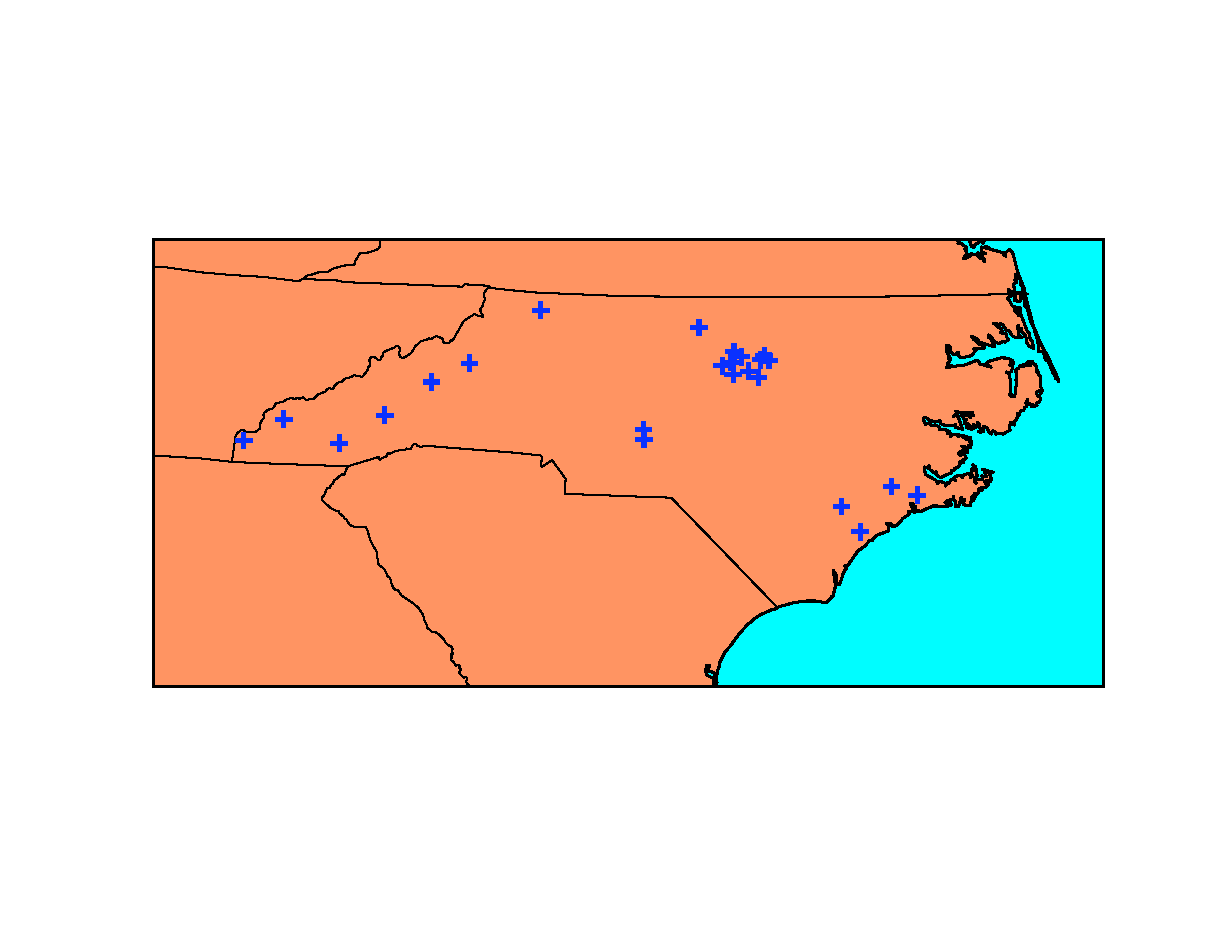
\includegraphics[width=0.6\columnwidth]{./figures/hands-on3/mapfig.pdf}
% \caption{Output of the mapex2.py module}
% \end{figure}
